\documentclass[aps,pra,reprint,superscriptaddress,nofootinbib,longbibliography,floatfix]{revtex4-2}

\usepackage[T1]{fontenc}
\usepackage{amsmath,amssymb,bm,mathtools}
\usepackage{graphicx}
\usepackage{dcolumn}
\usepackage{booktabs}
\usepackage{xcolor}
\usepackage{placeins}
\usepackage[protrusion=true,expansion=false]{microtype}
\usepackage[colorlinks=true,linkcolor=blue,citecolor=blue,urlcolor=blue]{hyperref}

\graphicspath{{figures/}}

\newcommand{\ii}{\mathrm{i}}
\newcommand{\ee}{\mathrm{e}}
\newcommand{\Del}{\Delta}
\newcommand{\Gam}{\Gamma}
\newcommand{\ph}{\varphi}
\newcommand{\thaone}{\theta_{a1}}
\newcommand{\thatwo}{\theta_{a2}}
\newcommand{\thbtwo}{\theta_{b2}}
\newcommand{\thbthree}{\theta_{b3}}
\newcommand{\Bthree}{\mathcal{B}_3}
\newcommand{\Poneplus}{P_{1+}}
\newcommand{\Poneminus}{P_{1-}}
\newcommand{\Pthreeplus}{P_{3+}}
\newcommand{\Pthreeminus}{P_{3-}}

\begin{document}

\title{Phase-controlled six-port single-photon scattering in a two-giant-atom three-waveguide node}

\author{Author Name}
\affiliation{School of Physics and Materials Science, Guangzhou University, Guangzhou 510006, China}

\date{\today}

\begin{abstract}
We study a single-photon scattering model in a waveguide-QED node formed by two giant atoms coupled to three one-dimensional waveguides.
The two atoms connect the three waveguides in series through a shared middle waveguide, producing a six-port scattering problem because a photon may enter from either side of any waveguide.
Using a real-space scattering formulation, we solve the boundary and atomic equations and assemble the complete $6\times6$ scattering matrix from six independently derived incident columns.
The direct matrix solution is unitary to numerical precision and provides an oracle for checking compact analytical formulas.
Local coupling phases act as interference controls that are absent in the corresponding small-atom reference, where the two far-waveguide output directions remain probabilistically indistinguishable.
For the giant-atom node, representative fixed-backbone parameter sets realize near-unit routing to selected output ports, while phase-space maps reveal both broad constructive basins and narrow near-resonant routes.
Reversing all local coupling phases gives the time-reversed scattering response, $T_{ij}(\theta)=T_{ji}(-\theta)$.
\end{abstract}

\maketitle

\section{Introduction}

The interaction between light and matter confined to one-dimensional continua is central to waveguide quantum electrodynamics (QED) \cite{Roy2017Colloquium,Gu2017MicrowavePhotonics}.
When an artificial atom couples to a waveguide at multiple spatially separated points---the giant-atom regime \cite{Kockum2014Designing,Kockum2018GiantAtoms}---propagation phases between coupling points become controllable scattering parameters.
These phase degrees of freedom enable effects without a direct small-atom analog, including frequency-dependent relaxation and Lamb shifts, decoherence-free atomic states, and non-Markovian scattering dynamics \cite{Kockum2018GiantAtomsReview,Kannan2020GiantAtom}.

For quantum-network applications, a central challenge is to route single photons among multiple output ports with high fidelity \cite{Zhou2008SinglePhotonRouter}.
Conventional small-atom routers often rely on chiral couplings or external driving to break reciprocity.
Giant-atom structures offer a complementary route by encoding routing instructions in the interference between spatially separated coupling channels.
Recent work on phase-controlled giant-molecule scattering has demonstrated that local coupling phases alone can realize targeted routing and asymmetric single-photon scattering without requiring chiral couplings \cite{Sun2025PhaseControlled}.

Here we study a two-giant-atom, three-waveguide node: atom $a$ couples to waveguides~1 and~2, atom $b$ couples to waveguides~2 and~3, and waveguide~2 acts as a shared bus (Fig.~\ref{fig:model}).
The six external ports---left and right directions on each waveguide---make this the minimal geometry in which a single photon can be flexibly routed among all three waveguides in both directions.
The system has two physically distinct incident configurations: edge incidence from waveguide~1 (or, by symmetry, waveguide~3), and middle incidence from the shared waveguide~2.
Within each configuration, the routing problem reduces to selecting among six available output channels.

Our aim is to derive the scattering amplitudes in closed analytical form and expose the algebraic structure behind the routing behavior.
We find that all scattering amplitudes---for both edge and middle incidence---share a common denominator $M$ whose pole structure encodes the collective two-atom resonance.
The amplitudes admit a compact $\eta$-form representation: each output is expressed through the atomic excitation amplitudes $\eta_a,\eta_b$ and elementary phase factors.
Three amplitudes ($r_1,t_1,r_2$) further reduce to factorized rational forms, while the remainder retain their $\eta$-form structure.
Many routing conditions reduce to simple phase-factor zeros, while the waveguide-2 outputs are governed by linear-combination zeros, providing a compact classification of representative routing mechanisms.

The paper is organized as follows.
Section~II introduces the model, Hamiltonian, and real-space scattering formalism, including the edge-incidence factorized amplitudes and the zero-condition covering classification.
Section~III visualizes the edge-incidence routing landscape under the fixed backbone $\Gamma=1,\theta_{a2}=\pi$.
Section~IV derives the middle-incidence amplitudes and uses them, together with the edge-incidence results and independently derived right-incidence columns, to construct the complete $6\times6$ scattering matrix.
Section~V discusses finite-delay extensions and directions for future work.

\section{Model and Hamiltonian}

\subsection{Model configuration}

The system consists of three infinite one-dimensional waveguides and two two-level giant atoms.
Atom $a$ couples to waveguide~1 at two points ($x=0$ and $x=l_1$) and to waveguide~2 at two points ($x=0$ and $x=l_2$).
Atom $b$ couples to waveguide~2 at the same two points as atom $a$, and to waveguide~3 at two points ($x=0$ and $x=l_3$).
The shared bus waveguide~2 thus mediates an effective interaction between the two atoms.

\begin{figure}[t]
  \centering
  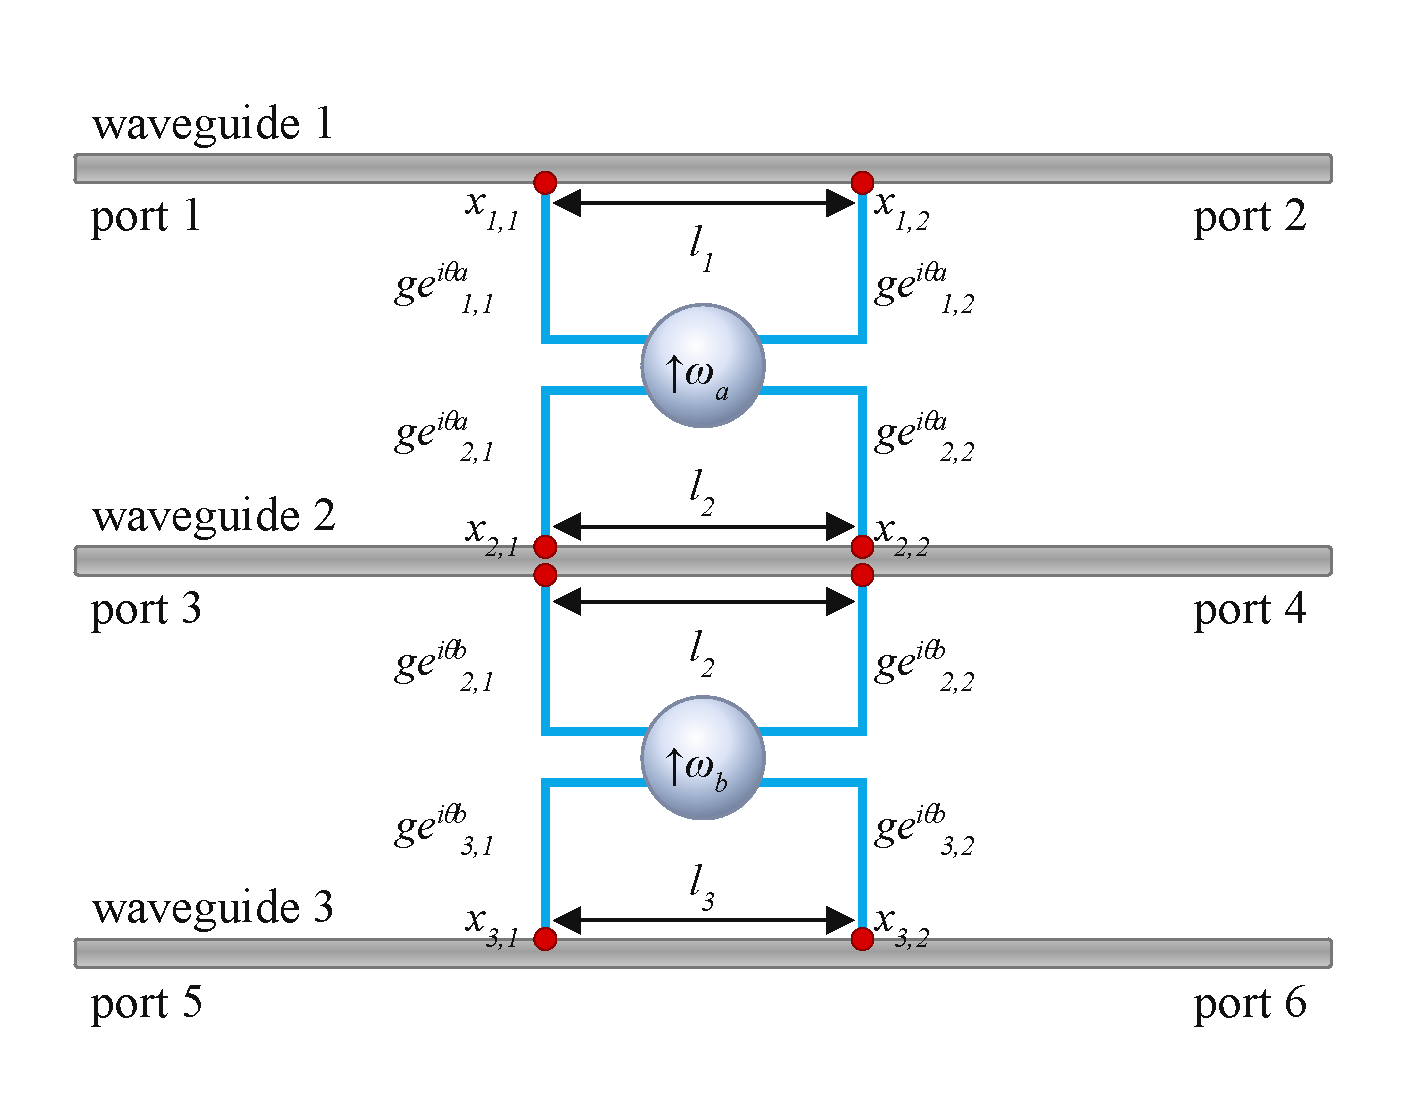
\includegraphics[width=\columnwidth]{fig1_system_schematic_vector_cropped.pdf}\\[2pt]
  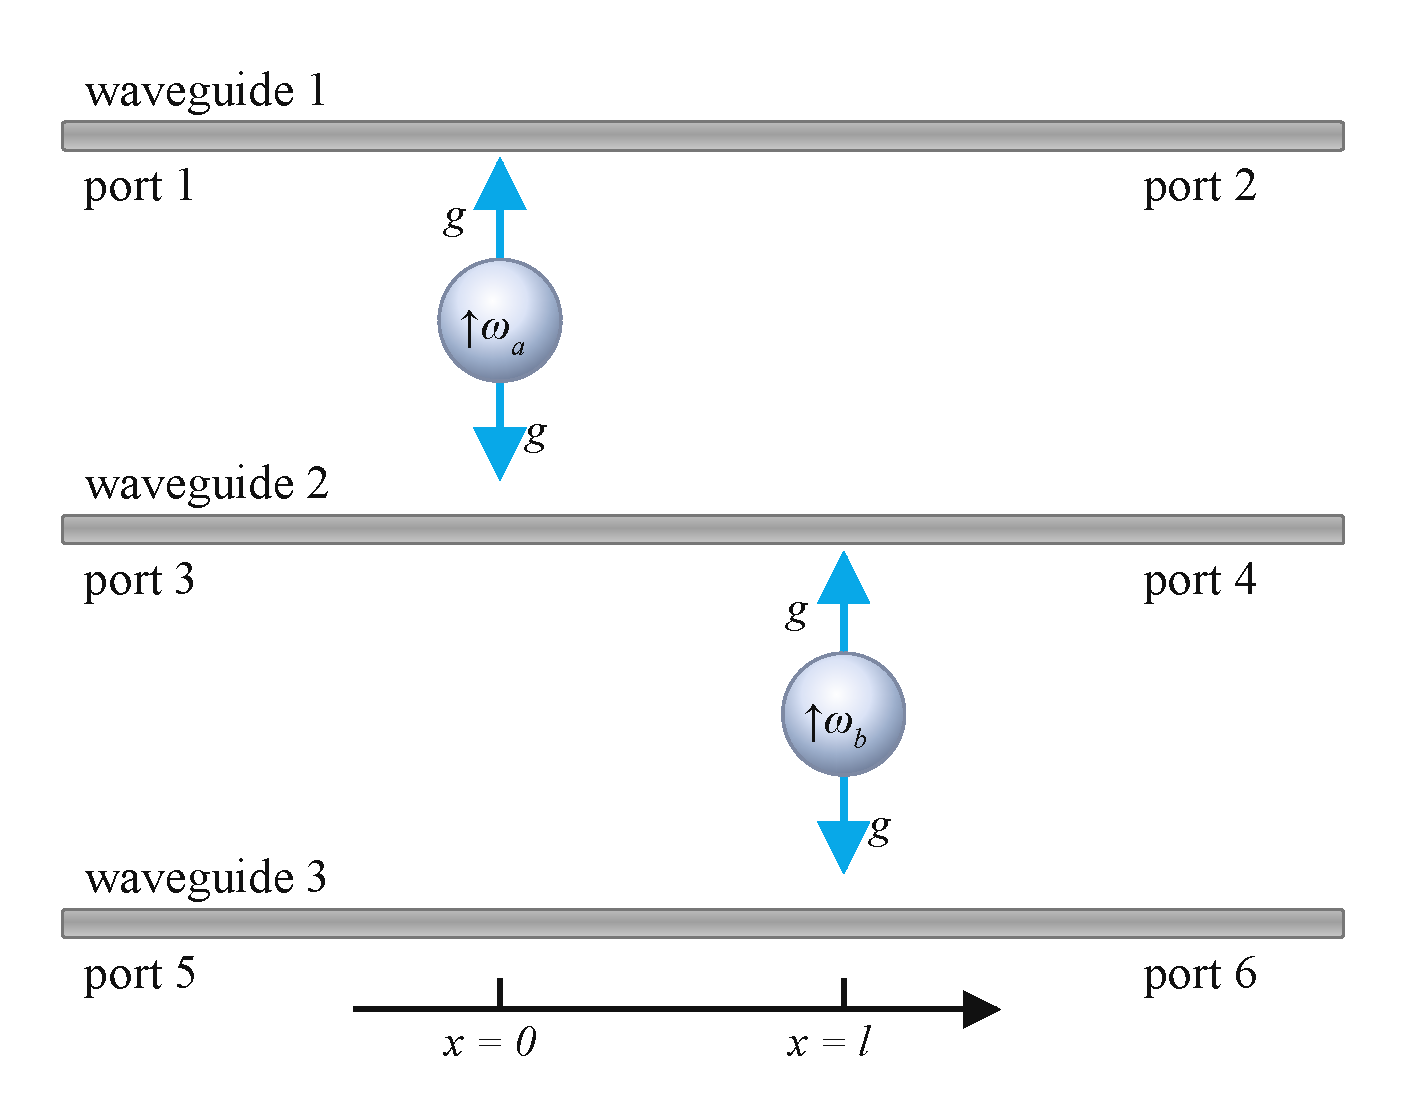
\includegraphics[width=0.92\columnwidth]{fig_small_atom_schematic_vector_cropped.pdf}
  \caption{Two-atom, three-waveguide six-port geometry.
  Top: giant-atom node studied in this work, where atom $a$ couples twice to waveguides~1 and~2, while atom $b$ couples twice to waveguides~2 and~3.
  Bottom: corresponding small-atom reference, in which each atom couples locally to its adjacent waveguides.
  For WG1-L incidence in the giant-atom node, the output amplitudes are $r_1$ (port~1), $t_1$ (port~2), $r_2$ (port~3), $t_2$ (port~4), $r_3$ (port~5), and $t_3$ (port~6).}
  \label{fig:model}
\end{figure}

The six external ports are labeled by the asymptotic propagation direction on each waveguide:
\begin{equation}
\begin{aligned}
(1,2,3,4,5,6)=(&\text{WG1-L},\text{WG1-R},\text{WG2-L},\\
&\text{WG2-R},\text{WG3-L},\text{WG3-R}),
\end{aligned}
\label{eq:ports}
\end{equation}
where ``L'' and ``R'' refer to the left- and right-moving output directions, respectively.
With this ordering, $S_{ij}$ denotes the output amplitude at port $i$ for a unit-amplitude input from port $j$.
With this convention, for WG1 left incidence the reflection amplitude $r_1$ exits through port~1 (WG1-L, left-moving) and the transmission amplitude $t_1$ exits through port~2 (WG1-R, right-moving).
The complete column vector for WG1-L incidence is therefore $\mathbf{s}^{(1)} = (r_1,\,t_1,\,r_2,\,t_2,\,r_3,\,t_3)^{\mathsf T}$.

\subsection{Hamiltonian and parameters}

In the rotating-wave approximation with linearized dispersion, the real-space Hamiltonian reads ($\hbar=1$)
\begin{subequations}
\label{eq:H}
\begin{align}
H &= H_{\rm at} + H_{\rm wg} + H_{\rm int},\\[2pt]
H_{\rm at} &= \sum_{m=a,b} \omega_m \sigma_m^+ \sigma_m^-,\\[2pt]
H_{\rm wg} &= \ii v_g \sum_{j=1}^3 \int dx\,
\bigl[L_j^\dagger(x)\partial_x L_j(x) - R_j^\dagger(x)\partial_x R_j(x)\bigr],\\[2pt]
H_{\rm int} &= \sum_{j=1,2} \int dx\, G_j^a(x)\,\sigma_a^+\bigl[L_j(x)+R_j(x)\bigr] \nonumber\\
&\quad + \sum_{j=2,3} \int dx\, G_j^b(x)\,\sigma_b^+\bigl[L_j(x)+R_j(x)\bigr] + \mathrm{H.c.},\\[2pt]
G_j^m(x) &= g\bigl[\ee^{\ii\theta^m_{j,1}}\delta(x) + \ee^{\ii\theta^m_{j,2}}\delta(x-l_j)\bigr].
\end{align}
\end{subequations}
Here $R_j^\dagger(x)$ and $L_j^\dagger(x)$ create right- and left-moving photons in waveguide $j$, $v_g$ is the group velocity, and $\sigma_m^\pm$ are the raising and lowering operators for atom $m$.
The coupling function $G_j^m(x)$ contains two local phases $\theta^m_{j,1}$ and $\theta^m_{j,2}$ at the two coupling points.
Only their difference
\begin{equation}
  \theta_{mj} = \theta^m_{j,2} - \theta^m_{j,1}
\end{equation}
enters the final scattering coefficients; we fix the gauge $\theta^m_{j,1}=0$ throughout.
The four independent phase differences are $\theta_{a1},\theta_{a2},\theta_{b2},\theta_{b3}$.
The propagation phase accumulated between the two coupling points on waveguide $j$ is
\begin{equation}
  \ph_j = k_j l_j .
\end{equation}

We define the photon--atom detuning $\Del \equiv \omega-\omega_a = \omega-\omega_b$ (the two atoms are taken to be degenerate), the waveguide-induced decay rate $\Gam \equiv g^2/v_g$, and the normalized atomic excitation amplitudes $\eta_m = g f_m / v_g$ ($m=a,b$).
It is also convenient to introduce the effective coupling parameter
\begin{equation}
  \tau_{mj} = 2\Gam\,\ee^{\ii\ph_j}\cos\theta_{mj},
\end{equation}
which combines the propagation phase and the local phase difference into a single complex quantity.

The single-excitation eigenstate of the total Hamiltonian takes the standard form
\begin{align}
|\Psi\rangle
=& \sum_{j=1}^3\int dx\,
\bigl[\Phi_{R,j}(x)R_j^\dagger(x)
+ \Phi_{L,j}(x)L_j^\dagger(x)\bigr]|\emptyset\rangle \nonumber\\
&+ f_a\sigma_a^+|\emptyset\rangle + f_b\sigma_b^+|\emptyset\rangle,
\label{eq:ansatz}
\end{align}
where $|\emptyset\rangle$ is the vacuum state of the waveguide fields and both atoms are in their ground states.
The photonic wavefunctions $\Phi_{R,j}(x)$ and $\Phi_{L,j}(x)$ are determined by the scattering boundary conditions together with the jump conditions at the coupling points, as detailed below.

\subsection{Scattering formulation: edge incidence}
\label{sec:edge}

The node supports two physically distinct incident configurations.
We first consider a photon incident from the left side of waveguide~1 (port~1).
The photonic wavefunctions take the piecewise form
\begin{subequations}
\label{eq:wg1_ansatz}
\begin{align}
\Phi_{R,1}(x) &= \ee^{\ii k_1 x}\bigl[\Theta(-x) + A\,\Theta(x)\Theta(l_1-x) \nonumber\\
&\qquad\qquad\qquad + t_1\,\Theta(x-l_1)\bigr],\\
\Phi_{L,1}(x) &= \ee^{-\ii k_1 x}\bigl[r_1\,\Theta(-x) + B\,\Theta(x)\Theta(l_1-x)\bigr],\\
\Phi_{R,2}(x) &= \ee^{\ii k_2 x}\bigl[C\,\Theta(x)\Theta(l_2-x) + t_2\,\Theta(x-l_2)\bigr],\\
\Phi_{L,2}(x) &= \ee^{-\ii k_2 x}\bigl[r_2\,\Theta(-x) + D\,\Theta(x)\Theta(l_2-x)\bigr],\\
\Phi_{R,3}(x) &= \ee^{\ii k_3 x}\bigl[E\,\Theta(x)\Theta(l_3-x) + t_3\,\Theta(x-l_3)\bigr],\\
\Phi_{L,3}(x) &= \ee^{-\ii k_3 x}\bigl[r_3\,\Theta(-x) + F\,\Theta(x)\Theta(l_3-x)\bigr],
\end{align}
\end{subequations}
where $\Theta(x)$ is the Heaviside step function.
The coefficients $A,B,C,D,E,F$ describe the photonic field inside the coupling regions, and $t_j,r_j$ are the transmission and reflection amplitudes on waveguide $j$.
Integrating the Schr\"{o}dinger equation $H|\Psi\rangle = E|\Psi\rangle$ across the coupling points yields 12 jump conditions relating these 12 waveguide variables.
Two additional atomic self-consistency equations determine the atomic excitation amplitudes $f_a,f_b$.
Together these equations form a closed $14\times14$ linear system,
\begin{equation}
\begin{aligned}
\mathcal{A}_1\mathbf{x}^{(1)}&=\mathbf{b}_1,\\
\mathbf{x}^{(1)}
&= (A,B,C,D,E,F,r_1,t_1,r_2,t_2,r_3,t_3,
\eta_a^{(1)},\eta_b^{(1)})^{\mathsf T},
\end{aligned}
\label{eq:linear_wg1}
\end{equation}
where the source vector $\mathbf{b}_1$ contains the unit incident field on waveguide~1.
The full set of 14 equations is given in Appendix~\ref{app:derivation}; solving this system analytically gives the six scattering amplitudes below.

\subsection{Factorized scattering amplitudes}

Solving the $14\times14$ system yields the common denominator
\begin{align}
M =& -2\Gam^2\cos(\thatwo-\thbtwo)
     - 4\Gam^2\ee^{2\ii\ph_2}
       \sin^2\frac{\thatwo-\thbtwo}{2} \nonumber\\
   & + \tau_{a1}\tau_{b2}
     + (\tau_{a1}+\tau_{a2})\tau_{b3} \nonumber\\
   & + (2\Gam-\ii\Del)(\tau_{a2}+\tau_{b2})
     + (4\Gam-\ii\Del)(\tau_{a1}+\tau_{b3}) \nonumber\\
   & + 14\Gam^2 - 8\ii\Gam\Del - \Del^2,
\label{eq:M}
\end{align}
and the six scattering amplitudes.
It is useful to first express the amplitudes through the atomic excitation amplitudes $\eta_a^{(1)},\eta_b^{(1)}$ obtained from the $14\times14$ system:
The superscript labels the incident port, not a power: $\eta_a^{(1)}$ and $\eta_b^{(1)}$ are the atomic excitation amplitudes driven by a unit input from port~1, while a different incident port gives a different source vector and hence different excitation amplitudes.
This $\eta$-form separates two ingredients that are otherwise mixed in long rational expressions: the atomic response of the two-emitter subsystem and the directional radiation factors into each output port.
\begin{subequations}
\label{eq:wg1_amps_eta}
\begin{align}
r_1 &= -\ii\eta_a^{(1)} P_{1-}, \label{eq:r1_eta}\\[2pt]
t_1 &= 1 - \ii\eta_a^{(1)} P_{1,a}^{R}, \label{eq:t1_eta}\\[2pt]
r_2 &= -\ii\bigl(\eta_a^{(1)} P_{2-}^a + \eta_b^{(1)} P_{2-}^b\bigr), \label{eq:r2_eta}\\[2pt]
t_2 &= -\ii\bigl(\eta_a^{(1)} P_{2,a}^{R} + \eta_b^{(1)} P_{2,b}^{R}\bigr), \label{eq:t2_eta}\\[2pt]
r_3 &= -\ii\eta_b^{(1)} P_{3-}, \label{eq:r3_eta}\\[2pt]
t_3 &= -\ii\eta_b^{(1)} P_{3,b}^{R}. \label{eq:t3_eta}
\end{align}
\end{subequations}
Here we use a systematic phase-factor notation to distinguish the source factor and the two output directions:
\begin{equation}
\begin{aligned}
P_{j,m}^{\rm src}&=1+\ee^{\ii(\ph_j+\theta_{mj})},\\
P_{j,m}^{L}&=1+\ee^{\ii(\ph_j-\theta_{mj})},\\
P_{j,m}^{R}&=1+\ee^{-\ii(\ph_j+\theta_{mj})},
\end{aligned}
\label{eq:Pnotation_wg1}
\end{equation}
so $P_{j,m}^{R}=(P_{j,m}^{\rm src})^*$, whereas $P_{j,m}^{L}$ is the left-output radiation factor.
For compactness we write $\Poneplus\equiv P_{1,a}^{\rm src}$, $\Poneminus\equiv P_{1,a}^{L}$, $\Pthreeplus\equiv P_{3,b}^{\rm src}$, and $\Pthreeminus\equiv P_{3,b}^{L}$.
The ballistic ``1'' in $t_1$ represents the transmitted photon that passes through without atomic interaction.

The atomic excitation amplitudes are obtained from the reduced $2\times2$ atomic subsystem:
\begin{subequations}
\label{eq:eta_wg1}
\begin{align}
\eta_a^{(1)} &= -\ii\Gam\,\Poneplus\,(\tau_{b2}+\tau_{b3}+4\Gam-\ii\Del)/M,\\[2pt]
\eta_b^{(1)} &= \frac{-\ii\Gam\Poneplus}{M\,P_{2-}^b}
\bigl[A_r - (\tau_{b2}+\tau_{b3}+4\Gam-\ii\Del)P_{2-}^a\bigr],
\end{align}
\end{subequations}
with the full derivation provided in Appendix~\ref{app:derivation}.
For reference, the $\eta$-form of Eqs.~\eqref{eq:wg1_amps_eta} reproduces the exhaustive rational expressions obtained by directly eliminating $\eta_a^{(1)},\eta_b^{(1)}$. After elimination, $r_1$, $t_1$, and $r_2$ recover the compact factorized forms
\begin{subequations}
\label{eq:wg1_factorized}
\begin{align}
t_1 &= N_{t_1}/M, \label{eq:t1_fact}\\[2pt]
r_1 &= -\Gam\,\Poneminus\Poneplus\,(\tau_{b2}+\tau_{b3}+4\Gam-\ii\Del)/M, \label{eq:r1_fact}\\[2pt]
r_2 &= -\Gam\,\Poneplus\,A_r/M, \label{eq:r2_fact}
\end{align}
\end{subequations}
The quantity $N_{t_1}$ is not an elementary interference factor; it is simply the full numerator of $t_1$, introduced to keep the main text compact, and is given explicitly in Appendix~\ref{app:t1}.
The eliminated form for $r_2$ has been verified to reduce to $-\Gamma\Poneplus A_r/M$.
By contrast, the previously tempting one-factor eliminated expressions for $t_2$, $t_3$, and $r_3$ do not pass the direct-oracle audit, so these channels are deliberately retained in the verified $\eta$-form of Eqs.~\eqref{eq:t2_eta}--\eqref{eq:t3_eta}.
The elementary phase factors entering Eqs.~\eqref{eq:wg1_amps_eta} are
\begin{subequations}
\label{eq:P}
\begin{align}
\Poneplus &= 1 + \ee^{\ii(\ph_1+\thaone)}, \qquad
\Poneminus = 1 + \ee^{\ii(\ph_1-\thaone)},\\
\Pthreeplus &= 1 + \ee^{\ii(\ph_3+\thbthree)}, \qquad
\Pthreeminus = 1 + \ee^{\ii(\ph_3-\thbthree)}.
\end{align}
\end{subequations}
Two composite interference factors control waveguide~2:
\begin{subequations}
\label{eq:AtAr}
\begin{align}
A_t &= \bigl(1+\ee^{\ii(\ph_2+\thatwo)}\bigr)(\tau_{b3}+2\Gam-\ii\Del) \nonumber\\
&\quad + \Gam\bigl(1-\ee^{2\ii\ph_2}\bigr)
        \bigl(1-\ee^{\ii(\thatwo-\thbtwo)}\bigr),\\
A_r &= \bigl(1+\ee^{\ii(\ph_2-\thatwo)}\bigr)(\tau_{b3}+2\Gam-\ii\Del) \nonumber\\
&\quad + \Gam\bigl(1-\ee^{2\ii\ph_2}\bigr)
        \bigl(1-\ee^{\ii(\thbtwo-\thatwo)}\bigr).
\end{align}
\end{subequations}
The bridge factor coupling waveguides~2 and~3 is
\begin{equation}
\Bthree = 1 + \ee^{\ii(\thatwo-\thbtwo)}
+ \ee^{\ii(\ph_2+\thatwo)} + \ee^{\ii(\ph_2-\thbtwo)}.
\label{eq:B3}
\end{equation}

Equations~\eqref{eq:wg1_factorized} reveal a factorized structure for the three amplitudes that simplify under $\eta$-elimination: $r_1$ contains the product $\Poneminus\Poneplus$, $r_2$ contains $\Poneplus A_r$, and $t_1$ requires the full numerator $N_{t_1}$. The remaining amplitudes $t_2$, $t_3$, $r_3$ are given in compact $\eta$-form by Eqs.~\eqref{eq:t2_eta}--\eqref{eq:t3_eta}, where the algebraic complexity resides in $\eta_a^{(1)},\eta_b^{(1)}$ and the directional output factors.

\subsection{Zero-condition covering}

The $\eta$-form of Eqs.~\eqref{eq:wg1_amps_eta} reveals that both atomic excitation amplitudes share the entrance factor $\Poneplus$ [see Eqs.~\eqref{eq:eta_wg1}]. Consequently $\Poneplus=0$ simultaneously kills five amplitudes ($r_1,r_2,t_2,r_3,t_3$), leaving only $t_1$ active. Beyond this global cover, each amplitude possesses individual zero conditions:
\begin{align}
Z(r_1)&: \Poneminus=0 \;\text{or}\; \Poneplus=0,\\
Z(t_2)&: \eta_a^{(1)}P_{2,a}^{R} + \eta_b^{(1)}P_{2,b}^{R}=0,\\
Z(r_2)&: \eta_a^{(1)}P_{2-}^{a} + \eta_b^{(1)}P_{2-}^{b}=0,\\
Z(t_3)&: \Poneplus=0 \;\text{or}\; P_{3,b}^{R}=0,\\
Z(r_3)&: \Poneplus=0 \;\text{or}\; P_{3-}=0.
\end{align}
The elementary phase-factor conditions are
\begin{subequations}
\begin{align}
\Poneplus=0 &\Longleftrightarrow \ph_1+\thaone = (2n+1)\pi,\\
\Poneminus=0 &\Longleftrightarrow \ph_1-\thaone = (2n+1)\pi,\\
P_{3,b}^{R}=0 &\Longleftrightarrow \ph_3+\thbthree = (2n+1)\pi,\\
P_{3-}=0 &\Longleftrightarrow \ph_3-\thbthree = (2n+1)\pi.
\end{align}
\end{subequations}
The conditions for $t_2$ and $r_2$ are linear combinations of $\eta_a^{(1)}$ and $\eta_b^{(1)}$ and do not factorize into single elementary zeros; they must be analyzed through the full atomic subsystem (see Appendix~\ref{app:derivation}).

Perfect routing to a target port requires selecting zero conditions that simultaneously suppress all five non-target ports while keeping the target amplitude and $M$ finite.
Table~\ref{tab:zero_coverings} summarizes the representative covering strategies.

\begin{table}[!htbp]
\caption{Representative sufficient zero-condition coverings for waveguide-1 edge incidence. Conditions $C_2^t$ and $C_2^r$ denote the linear-combination zeros $\eta_a^{(1)}P_{2,a}^{R}+\eta_b^{(1)}P_{2,b}^{R}=0$ and $\eta_a^{(1)}P_{2-}^{a}+\eta_b^{(1)}P_{2-}^{b}=0$, respectively. The table gives constructive coverings used in this work and is not a necessary-and-sufficient classification of all mathematical solutions.}
\label{tab:zero_coverings}
\centering
\resizebox{\columnwidth}{!}{%
\begin{tabular}{clll}
Target & Required non-target zeros & Target-preserving conditions & Status \\
\hline
$T_1$ & $\Poneplus=0$ & $M\neq0$ & Exact sufficient route \\
$R_1$ & $N_{t_1}=0,\ C_2^t=0,\ C_2^r=0,\ r_3=t_3=0$ & $\Poneplus\Poneminus\neq0,\ M\neq0$ & Composite route \\
$T_2$ & $N_{t_1}=0,\ \Poneminus=0,\ C_2^r=0,\ r_3=t_3=0$ & $C_2^t\neq0,\ M\neq0$ & Composite route \\
$R_2$ & $N_{t_1}=0,\ \Poneminus=0,\ C_2^t=0,\ r_3=t_3=0$ & $C_2^r\neq0,\ M\neq0$ & Composite route \\
$T_3$ & $N_{t_1}=0,\ \Poneminus=0,\ C_2^t=0,\ C_2^r=0,\ P_{3-}=0$ & $P_{3,b}^{R}\neq0,\ \Poneplus\neq0,\ M\neq0$ & Near-resonant representative route \\
$R_3$ & $N_{t_1}=0,\ \Poneminus=0,\ C_2^t=0,\ C_2^r=0,\ P_{3,b}^{R}=0$ & $P_{3-}\neq0,\ \Poneplus\neq0,\ M\neq0$ & Near-resonant representative route \\
\end{tabular}%
}
\end{table}

The covering classification naturally separates the six routing channels into three mechanism classes.
\textbf{Direct phase-zero route ($T_1$).}
The condition $\Poneplus=0$ simultaneously covers all five non-target ports, leaving only the self-transmission $t_1$ active.
Provided $M\neq0$, probability conservation guarantees $T_1=1$.
This is the cleanest mechanism: a single phase condition on $\ph_1+\thaone$ achieves perfect routing.

\textbf{Composite-interference routes ($R_1,T_2,R_2$).}
These channels require multiple simultaneous conditions---suppressing $t_1$ through its numerator, closing the waveguide-2 outputs through the linear-combination conditions $C_2^t$ and/or $C_2^r$, and suppressing the far waveguide by driving $\eta_b^{(1)}\to0$.
The number of constraints approaches the number of available parameters, making these routes exact or near-exact.

\textbf{Near-resonant singular routes ($T_3,R_3$).}
Routing to waveguide~3 is the most constrained case.
It requires entrance locking via $\Poneminus=0$ (since $\Poneplus=0$ would also kill the target), waveguide-2 closure via $C_2^t=C_2^r=0$, and direction selectivity on waveguide~3 through $P_{3,b}^{R}=0$ or $P_{3-}=0$.
At strict resonance $\Del=0$, the waveguide-2 closure conditions force degeneracy between the two waveguide-3 directions; a small nonzero detuning $\Del$ breaks this degeneracy at linear order, enabling directional selection.
The optimal detuning scale for the representative branch is $|\Del|/\Gam\sim 4.6\times10^{-3}$, consistent with the near-resonant character of this mechanism: a small but finite detuning is required to break the directional degeneracy, yet it must remain within the resonance window.

\section{Fixed-backbone edge-incidence routing landscape}
\label{sec:routing}

The zero-condition covering analysis of Sec.~\ref{sec:edge} is independent of any particular parameter choice.
To illustrate the routing mechanisms concretely, we fix the representative branch
\begin{equation}
  \boxed{\Gam=1,\qquad \thatwo=\pi,}
\end{equation}
which reduces the free parameter space to seven dimensions $(\Delta,\thaone,\thbtwo,\thbthree,\ph_1,\ph_2,\ph_3)$.
All angular parameters are quoted in units of $\pi$ below.

\subsection{Phase-space routing maps}

Figure~\ref{fig:phase_maps} displays two-dimensional slices through the seven-dimensional routing landscape around the high-transmission basins identified by the zero-condition coverings of Table~\ref{tab:zero_coverings}.
Figure~\ref{fig:phase_maps} shows four representative phase-space maps rather than all six target ports.
This choice follows the symmetry structure of the fixed-backbone problem: $T_2$ and $R_2$ form a direction-related pair, and $T_3$ and $R_3$ form a corresponding far-waveguide pair.
Because $T_2/R_2$ and $T_3/R_3$ form direction-related pairs under the fixed-backbone symmetry, the main figure shows $T_2$ and $T_3$ as representatives, while the corresponding $R_2$ and $R_3$ data are retained in Table~\ref{tab:opt} and the online repository.
The purpose of Fig.~\ref{fig:phase_maps} is not to enumerate every optimized target, but to compare the distinct routing mechanisms: direct self-transmission, same-waveguide reflection, shared-waveguide routing, and far-waveguide routing.
The plotted coordinates are chosen channel by channel so that the relevant structure is visible: broad routes are shown on full or seam-centered phase windows, while the remote waveguide-3 representative route requires a magnified near-resonant window.
All panels use the same probability color scale, so the areas of the high-fidelity regions can be compared directly.
The remaining parameters are held at their optimized values listed in Appendix~\ref{app:opt}, where the full six-target numerical record is preserved.

\begin{figure*}[!htbp]
  \centering
  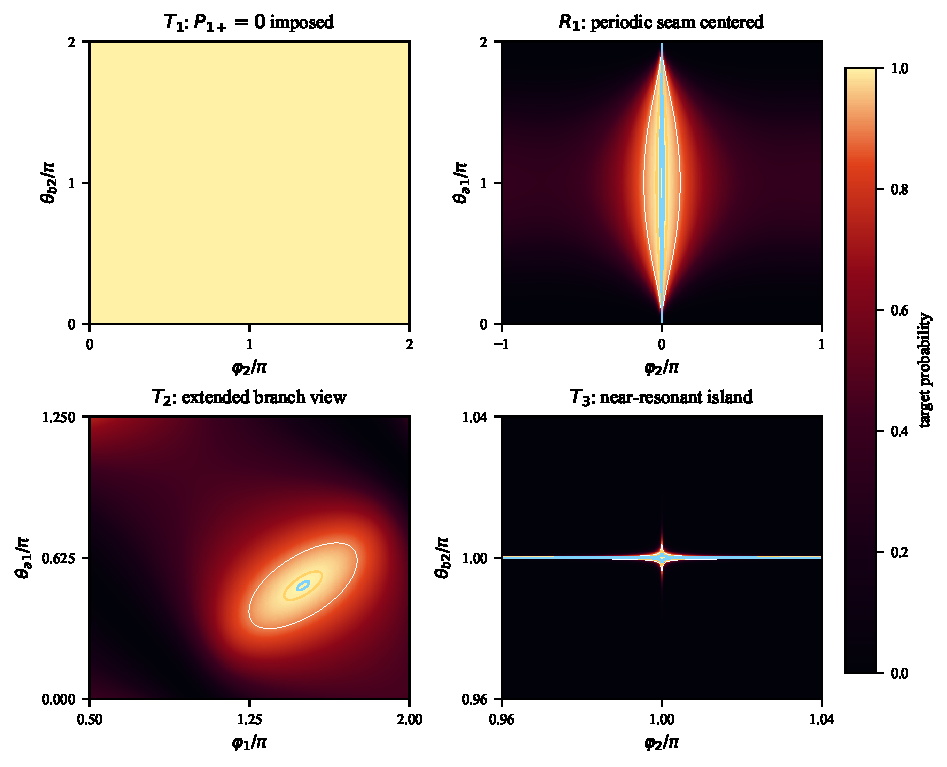
\includegraphics[width=0.96\textwidth]{fig_phase_routing_maps.pdf}
  \caption{Representative phase-coordinate routing landscapes for four fixed-backbone routing mechanisms under waveguide-1 edge incidence.
  The $T_1$ panel imposes the sufficient entrance condition $\Poneplus=0$ and scans the unrelated phases $(\varphi_2,\theta_{b2})$, showing that this condition is robust over a broad transverse parameter range rather than a fine-tuned point.
  The $R_1$ panel is recentered at the periodic seam so that the two edge features join into one continuous high-transmission region.
  The $T_2$ panel uses an extended branch window large enough to show the boundary of the high-fidelity island around the correlated branch neighborhood introduced below.
  The $T_3$ panel uses a magnified near-resonant window because the far-waveguide high-fidelity region is much narrower on the full phase torus.
  Contours mark $P=0.9$, $0.99$, and $0.999$ where visible.
  These two-dimensional cuts demonstrate sufficient high-probability routes around representative optima; in particular, the $T_1$ panel is a sufficiency test for $\Poneplus=0$, not a necessity proof.
  The complete six-target optimized parameter record is given in Table~\ref{tab:opt}; the symmetry-related $R_2$ and $R_3$ maps are retained in the repository all-target figure.}
  \label{fig:phase_maps}
\end{figure*}

The $T_1$ panel is particularly instructive: after fixing one representative point on the direct phase-zero condition $\ph_1+\thaone=(2n+1)\pi$ ($\Poneplus=0$), it scans the unrelated parameters $\varphi_2$ and $\theta_{b2}$ over the full $0$--$2\pi$ range.
The resulting near-unit plateau confirms that this entrance-interference condition suppresses the five non-target amplitudes without requiring simultaneous tuning of the downstream phases.
This condition is not claimed to be the only mathematical route to $T_1=1$; it is the simplest constructive route because it suppresses all five non-target amplitudes at once.
Residual variation in the panel is controlled by the common denominator $M$ and marks the finite exceptional set where the scattering problem approaches a pole or numerical singularity.

The $T_2$ panel exhibits a compact high-probability island, consistent with the composite-interference mechanism: this representative shared-waveguide channel requires the simultaneous satisfaction of multiple zero conditions, leaving a lower-dimensional solution manifold.
The $R_2$ map is omitted from the main figure because it is symmetry-related to $T_2$ and does not introduce a distinct routing class.
The $T_3$ panel shows a very narrow near-resonant ridge, reflecting the singular nature of the waveguide-3 routing mechanism discussed in Sec.~\ref{sec:edge}; the symmetry-related $R_3$ map is likewise omitted from the main figure and retained only in the full numerical record.
The complete set of six optimized parameter sets in Table~\ref{tab:opt} is therefore a numerical record, whereas Fig.~\ref{fig:phase_maps} is a representative mechanism comparison.

\subsection{Mechanism-guided basin comparison}

The representative landscapes in Fig.~\ref{fig:phase_maps} show where high routing probability occurs, but they do not by themselves explain how different mechanisms shape the local high-fidelity basin.
Figure~\ref{fig:branch_verification} therefore compares three representative nontrivial routes, $R_1$, $T_2$, and $T_3$, under two kinds of two-parameter scans: an unconstrained local scan around the optimized point and a mechanism-guided scan.
The symmetry-related $R_2$ and $R_3$ channels are omitted from this main mechanism comparison for the same reason they are omitted from Fig.~\ref{fig:phase_maps}: they do not introduce additional mechanism classes under the fixed-backbone symmetry and are retained in Table~\ref{tab:opt} and the online repository.

Only the $T_2$ row uses a closed analytic correlated branch.
For the $T_2$ route, the optimized point lies close to the following sufficient branch.
Writing phases in units of $\pi$, one representative branch is
\begin{equation}
\begin{aligned}
\mathcal{C}_2(q):\quad&
\ph_2/\pi=1-q,\qquad
\ph_3/\pi=0,\qquad
\thbthree/\pi=1,\\
&\ph_1/\pi=\frac{3}{2}+\frac{3q}{2},\qquad
\thaone/\pi=\frac{1}{2}+\frac{3q}{2},\\
&\Del/\Gam=2\sin(\pi q),
\end{aligned}
\label{eq:C2_branch}
\end{equation}
with $\thbtwo/\pi=q$ for one $T_2$ branch and a symmetry-related choice for $R_2$.
This relation should be read as a constructive sufficient path through parameter space rather than as a uniqueness statement.

For the $R_1$ and $T_3$ rows no analogous analytic branch is claimed.
Instead, the guided scans are numerical continuations performed with the direct $14\times14$ oracle.
For $R_1$, the direct-oracle continuation recenters the local scan by optimizing $\theta_{a1}$ for each displacement of $\varphi_2$, representing a same-waveguide composite-interference route.
For $T_3$, the guided scan recenters the detuning for each displacement of $\varphi_2$, representing the near-resonant far-waveguide route.
These numerical continuations are not proofs of uniqueness; they are local mechanism-guided cuts that show how the verified zero-condition mechanisms organize the high-fidelity basins.

\begin{figure*}[!htbp]
  \centering
  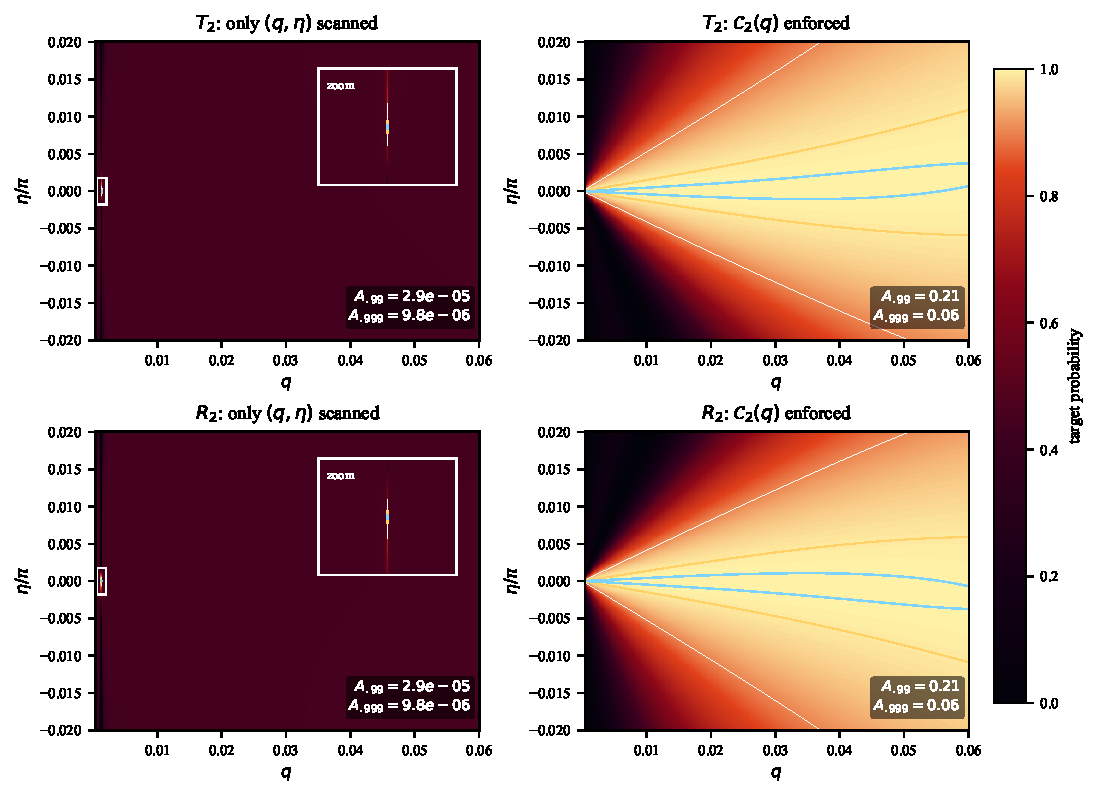
\includegraphics[width=0.96\textwidth]{fig_constructive_branch_verification.pdf}
  \caption{Representative mechanism comparison for nontrivial waveguide-1 edge-incidence routes.
  Rows show $R_1$ (same-waveguide composite reflection), $T_2$ (shared-waveguide routing), and $T_3$ (near-resonant far-waveguide routing).
  Left column: unconstrained local two-parameter scans around the optimized point.
  Right column: mechanism-guided scans.
  The $T_2$ row imposes the analytic correlated branch $\mathcal{C}_2(q)$ defined in Eq.~\eqref{eq:C2_branch}.
  The $R_1$ row uses direct-oracle numerical continuation of $\theta_{a1}$ around the optimized composite route, and the $T_3$ row uses direct-oracle detuning-guided continuation around the near-resonant route; no analytic $R_1$ or $T_3$ branch is assumed.
  All panels use the same probability color scale; contours mark $P=0.9$, $0.99$, and $0.999$ where visible.
  The displayed area fractions compare the high-fidelity basins for representative mechanisms rather than enumerating all six output channels.}
  \label{fig:branch_verification}
\end{figure*}

\subsection{Detuning sensitivity of near-resonant routes}

The near-resonant waveguide-3 channels are also unusually sensitive to detuning.
At strict resonance, the two waveguide-3 output directions are degenerate; a small but nonzero detuning breaks this degeneracy and selects one direction.
Figure~\ref{fig:detuning_window} illustrates this point for a representative $T_3$ solution.
The left panel shows that the high-fidelity window is narrow in $\Delta$, while the right panel compares the best target probabilities when $\Delta$ is optimized with those obtained after forcing $\Delta=0$.

\begin{figure*}[!htbp]
  \centering
  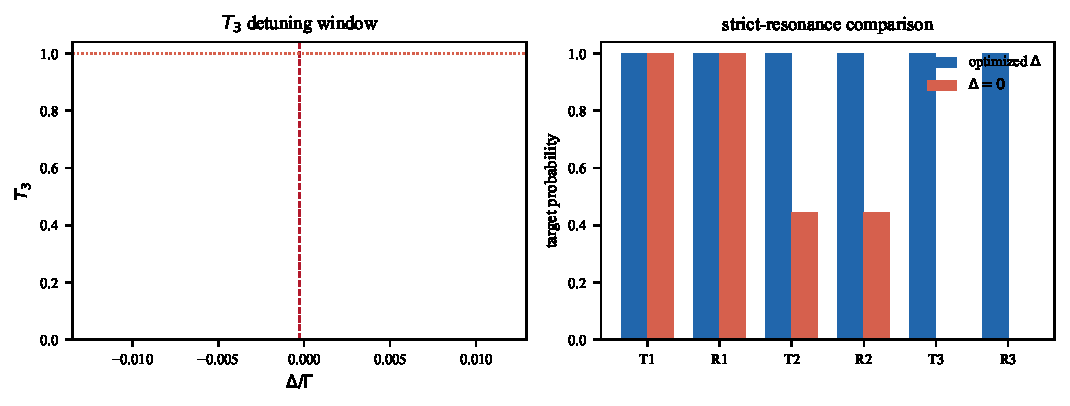
\includegraphics[width=0.9\textwidth]{fig6_detuning_degeneracy.pdf}
  \caption{Detuning sensitivity of the near-resonant waveguide-3 routing mechanism.
  Left: a representative $T_3$ line shape near the optimal detuning $\Delta_\ast$; the dashed line marks $T_3=0.999$.
  Right: comparison between optimizing $\Delta$ freely and imposing strict resonance $\Delta=0$.
  The waveguide-3 channels lose directional selectivity at strict resonance, consistent with the degeneracy argument in Sec.~\ref{sec:edge}.}
  \label{fig:detuning_window}
\end{figure*}

\subsection{Small-atom reference: absence of independent directional phase zeros}

To clarify the role of the giant-atom phase degrees of freedom, we briefly contrast the results above with the corresponding small-atom node.
In the small-atom limit, each atom couples to its waveguides at a single point: atom $a$ at $x=0$ on waveguides~1 and~2, atom $b$ at $x=l$ on waveguides~2 and~3.
The only propagation phase is $\phi=k_2l=k_3l$, and no local phase differences $\theta_{mj}$ exist.
We use the same definitions $\Gam=g^2/v_g$ and $\Del=\omega-\omega_a=\omega-\omega_b$ as in the giant-atom model.
Solving the same real-space scattering problem yields the six small-atom amplitudes.
The far-waveguide outputs are particularly instructive:
\begin{subequations}
\begin{align}
t_3^s &= \frac{\Gam^2}{D_s},\\
r_3^s &= \frac{\ee^{2\ii\phi}\Gam^2}{D_s},
\end{align}
\end{subequations}
with
\begin{equation}
  D_s = -4\Gam^2 + \ee^{2\ii\phi}\Gam^2 + 4\ii\Gam\Del + \Del^2.
\end{equation}
Consequently,
\begin{equation}
  |t_3^s|^2 = |r_3^s|^2,
\end{equation}
i.e., the two output directions on waveguide~3 are \emph{probabilistically indistinguishable} within this symmetric small-atom reference model.
No choice of $\phi$ or $\Del$ can make $|t_3^s|^2\neq|r_3^s|^2$.

In contrast, the giant-atom far-waveguide amplitudes [Eqs.~\eqref{eq:r3_eta}--\eqref{eq:t3_eta}] are proportional to two \emph{independent} phase factors,
\begin{equation}
  t_3 \propto P_{3,b}^{R} = 1+\ee^{-\ii(\ph_3+\thbthree)},\qquad
  r_3 \propto P_{3-} = 1+\ee^{\ii(\ph_3-\thbthree)},
\end{equation}
whose zeros can be controlled independently through the local phase difference $\thbthree$.
The small-atom node lacks this directional selectivity because all propagation accumulates in the single phase $\phi$, which factors out as a common modulus in $|t_3^s|^2$ and $|r_3^s|^2$.
This small-atom reference is included only to highlight the directional phase selectivity of the giant-atom node.

\section{Middle-incident scattering and the six-port matrix}
\label{sec:wg2}

\subsection{Motivation}

The edge-incidence amplitudes of Sec.~\ref{sec:edge} provide one column of the $6\times6$ scattering matrix (column~1 for WG1-L incidence, and by symmetry column~5 for WG3-L incidence).
To complete the left-incidence description of the node we also need the response to a photon entering from the middle waveguide~2 (port~3).
This middle-incidence configuration is physically distinct because the incident field drives both atoms simultaneously through their shared coupling to waveguide~2, rather than a single atom as in the edge case.

\subsection{Scattering ansatz for waveguide-2 incidence}

For a photon incident from the left of waveguide~2, the ansatz is obtained from Eq.~\eqref{eq:wg1_ansatz} by moving the unit incident amplitude from $\Phi_{R,1}$ to $\Phi_{R,2}$:
\begin{subequations}
\label{eq:wg2_ansatz}
\begin{align}
\Phi_{R,1}(x) &= \ee^{\ii k_1 x}\bigl[\tilde A\,\Theta(x)\Theta(l_1-x) + \tilde t_1\,\Theta(x-l_1)\bigr],\\
\Phi_{L,1}(x) &= \ee^{-\ii k_1 x}\bigl[\tilde r_1\,\Theta(-x) + \tilde B\,\Theta(x)\Theta(l_1-x)\bigr],\\
\Phi_{R,2}(x) &= \ee^{\ii k_2 x}\bigl[\Theta(-x) + \tilde C\,\Theta(x)\Theta(l_2-x) \nonumber\\
&\qquad\qquad\qquad + \tilde t_2\,\Theta(x-l_2)\bigr],\\
\Phi_{L,2}(x) &= \ee^{-\ii k_2 x}\bigl[\tilde r_2\,\Theta(-x) + \tilde D\,\Theta(x)\Theta(l_2-x)\bigr],\\
\Phi_{R,3}(x) &= \ee^{\ii k_3 x}\bigl[\tilde E\,\Theta(x)\Theta(l_3-x) + \tilde t_3\,\Theta(x-l_3)\bigr],\\
\Phi_{L,3}(x) &= \ee^{-\ii k_3 x}\bigl[\tilde r_3\,\Theta(-x) + \tilde F\,\Theta(x)\Theta(l_3-x)\bigr].
\end{align}
\end{subequations}
Compared with Eq.~\eqref{eq:wg1_ansatz}, the only physical change is where the incoming unit-amplitude wave is placed.
For WG1 incidence the incoming term is the ``$1$'' in $\Phi_{R,1}$ before the first coupling point; for WG2 incidence it is the ``$1$'' in $\Phi_{R,2}$ before the first coupling point.
The Hamiltonian, coupling phases, and jump rules at the six coupling points are unchanged.
Thus the 14 equations have the same left-hand-side coefficients as in the edge-incidence problem: the unknown internal amplitudes, output amplitudes, and atomic amplitudes enter with the same phase factors.
What changes are the constant source terms generated by the incoming photon.
Equivalently, in the matrix form $\mathcal{A}\mathbf{x}=\mathbf{b}$, the matrix $\mathcal{A}$ is the same and the source vector $\mathbf{b}$ is changed.
This is why the middle-incidence amplitudes share the same denominator $M$ as Eq.~\eqref{eq:M}.

\subsection{Scattering amplitudes in compact form}

Solving the 12 jump conditions for the internal waveguide amplitudes in terms of $\eta_a^{(3)},\eta_b^{(3)}$ (see Appendix~\ref{app:derivation} for details) and substituting into the remaining relations yields the six scattering amplitudes:
\begin{subequations}
\label{eq:wg2_amps}
\begin{align}
\tilde t_1 &= -\ii\eta_a^{(3)} P_{1,a}^{R}, \qquad
\tilde r_1 = -\ii\eta_a^{(3)} P_{1,a}^{L},\\[2pt]
\tilde t_2 &= 1 - \ii\eta_a^{(3)} P_{2,a}^{R} - \ii\eta_b^{(3)} P_{2,b}^{R},\\[2pt]
\tilde r_2 &= -\ii\eta_a^{(3)} P_{2,a}^{L} - \ii\eta_b^{(3)} P_{2,b}^{L},\\[2pt]
\tilde t_3 &= -\ii\eta_b^{(3)} P_{3,b}^{R}, \qquad
\tilde r_3 = -\ii\eta_b^{(3)} P_{3,b}^{L}.
\end{align}
\end{subequations}
Here we have introduced a systematic phase-factor notation to distinguish the three physically distinct roles played by phase factors in the scattering problem:
\begin{equation}
\begin{aligned}
P_{j,m}^{\rm src} &= 1+\ee^{\ii(\ph_j+\theta_{mj})},\\
P_{j,m}^{R} &= 1+\ee^{-\ii(\ph_j+\theta_{mj})},\\
P_{j,m}^{L} &= 1+\ee^{\ii(\ph_j-\theta_{mj})},
\end{aligned}
\label{eq:Pnotation}
\end{equation}
corresponding respectively to the source driving factor (coupling of the incident field to the atom), the right-moving output factor, and the left-moving output (reflection) factor.
Note that $P_{j,m}^{R} = (P_{j,m}^{\rm src})^*$, while $P_{j,m}^{L}$ is an independent factor.

The term ``$1$'' in $\tilde t_2$ represents the ballistic transmission background---a photon that passes through waveguide~2 without interacting with either atom.
The actual value of $\tilde t_2$ is modified from unity by the scattering contributions proportional to $\eta_a^{(3)}$ and $\eta_b^{(3)}$.

\subsection{Atomic excitation amplitudes}

The atomic amplitudes $\eta_a^{(3)},\eta_b^{(3)}$ are obtained by substituting the jump-condition relations into the atomic self-consistency equations.
The $14\times14$ linear system reduces to a $2\times2$ system for $(\eta_a^{(3)},\eta_b^{(3)})$, whose solution factorizes in terms of the \emph{same} composite factors that appear in the edge-incidence result:
\begin{subequations}
\label{eq:eta_wg2}
\begin{align}
\eta_a^{(3)} &= -\ii\Gam\frac{A_t}{M},\\[2pt]
\eta_b^{(3)} &= -\ii\Gam\frac{A_t^b}{M},
\end{align}
\end{subequations}
where $A_t$ is given by Eq.~\eqref{eq:AtAr} and $A_t^b$ is its $a\leftrightarrow b$ symmetric counterpart,
\begin{align}
A_t^b = \bigl(1+\ee^{\ii(\ph_2+\thbtwo)}\bigr)(\tau_{a1}+2\Gam-\ii\Del)
       + \Gam\bigl(1-\ee^{2\ii\ph_2}\bigr) \nonumber\\
       \times\bigl(1-\ee^{\ii(\thbtwo-\thatwo)}\bigr).
\label{eq:Atb}
\end{align}
The complete derivation, including the $2\times2$ reduction and the verification by back-substitution into all 14 Schr\"{o}dinger equations, is presented in Appendix~\ref{app:derivation}.

Substituting Eqs.~\eqref{eq:eta_wg2} into Eqs.~\eqref{eq:wg2_amps} gives the waveguide-2 scattering amplitudes in fully explicit rational form:
\begin{subequations}
\label{eq:wg2_explicit}
\begin{align}
\tilde t_1 &= -\Gam\,P_{1,a}^{R}\,A_t/M, \qquad
\tilde r_1 = -\Gam\,P_{1,a}^{L}\,A_t/M,\\[2pt]
\tilde t_2 &= 1 - \Gam\,(P_{2,a}^{R}A_t + P_{2,b}^{R}A_t^b)/M,\\[2pt]
\tilde r_2 &= -\Gam\,(P_{2,a}^{L}A_t + P_{2,b}^{L}A_t^b)/M,\\[2pt]
\tilde t_3 &= -\Gam\,P_{3,b}^{R}\,A_t^b/M, \qquad
\tilde r_3 = -\Gam\,P_{3,b}^{L}\,A_t^b/M.
\end{align}
\end{subequations}

Equations~\eqref{eq:wg2_amps}--\eqref{eq:wg2_explicit} should be read in two steps.
First, once the atomic excitation amplitudes $\eta_a^{(3)}$ and $\eta_b^{(3)}$ are known, each output amplitude is obtained by multiplying the relevant atomic amplitude by the phase factor for that output direction.
For example, emission from atom $a$ into the right side of waveguide~1 gives $\tilde t_1\propto \eta_a^{(3)}P_{1,a}^{R}$, while emission into the left side gives $\tilde r_1\propto \eta_a^{(3)}P_{1,a}^{L}$.
The middle-waveguide outputs contain contributions from both atoms because both atoms couple to waveguide~2.
Second, the atomic amplitudes themselves are driven by the incident photon through the two composite numerators $A_t$ and $A_t^b$.
Here $A_t$ is the effective drive of atom $a$ after all interference paths through waveguide~2 are included, $A_t^b$ is the corresponding drive of atom $b$, and $M$ is the common response denominator of the coupled two-atom system.
Thus the formula has a simple physical structure: source interference determines $\eta_a^{(3)}$ and $\eta_b^{(3)}$, and these atomic excitations then radiate into the six output ports with direction-dependent phase factors.

\subsection{\texorpdfstring{Construction of the complete $6\times6$ scattering matrix}{Construction of the complete 6x6 scattering matrix}}

The three independent left-incidence column vectors, ordered according to the port convention of Eq.~\eqref{eq:ports}, are
\begin{equation}
\begin{aligned}
\mathbf{s}^{(1)} &= (r_1,\, t_1,\, r_2,\, t_2,\, r_3,\, t_3)^{\mathsf T},\\
\mathbf{s}^{(3)} &= (\tilde r_1,\, \tilde t_1,\, \tilde r_2,\, \tilde t_2,\, \tilde r_3,\, \tilde t_3)^{\mathsf T},\\
\mathbf{s}^{(5)} &= (\hat r_1,\, \hat t_1,\, \hat r_2,\, \hat t_2,\, \hat r_3,\, \hat t_3)^{\mathsf T},
\end{aligned}
\label{eq:three_cols}
\end{equation}
corresponding to incidence from the left side of waveguides~1, 2, and 3, respectively.
Column~1 is given by Eqs.~\eqref{eq:wg1_amps_eta} together with Eqs.~\eqref{eq:eta_wg1}, column~3 by Eqs.~\eqref{eq:wg2_amps} together with Eqs.~\eqref{eq:eta_wg2}, and column~5 follows from column~1 by the $a\leftrightarrow b$ atom-exchange symmetry:
\begin{equation}
\begin{aligned}
\theta_{a1}&\leftrightarrow\theta_{b3},&
\theta_{a2}&\leftrightarrow-\theta_{b2},&
\theta_{b2}&\leftrightarrow-\theta_{a2},\\
\theta_{b3}&\leftrightarrow\theta_{a1},&
\ph_1&\leftrightarrow\ph_3,
\end{aligned}
\label{eq:symmetry}
\end{equation}
followed by remapping the output port order $(r_1,t_1,r_2,t_2,r_3,t_3)\to(\hat r_3,\hat t_3,\hat r_2,\hat t_2,\hat r_1,\hat t_1)$.

The remaining three right-incidence columns $\mathbf{s}^{(2)},\mathbf{s}^{(4)},\mathbf{s}^{(6)}$ are obtained by independently solving the same $14\times14$ linear system with the appropriate incident boundary conditions (a left-moving photon entering from the right side of each waveguide). The $\eta$ form for these columns is constructed analogously to Eqs.~\eqref{eq:wg1_amps_eta} and~\eqref{eq:wg2_amps}; the complete set of machine-readable $\eta$-form expressions for all six ports is included in the online repository prepared for this work.

Importantly, the system is \emph{not} reciprocal in the sense $S=S^{\mathsf T}$ when local coupling phases are nonzero. The phase-reversed configuration is the time-reversal (TR) partner of the original system, which for the scattering matrix implies the probability-level partner relation
\begin{equation}
  T_{ij}(\theta_{a1},\theta_{a2},\theta_{b2},\theta_{b3})
  = T_{ji}(-\theta_{a1},-\theta_{a2},-\theta_{b2},-\theta_{b3}),
  \label{eq:tr_partner}
\end{equation}
where $T_{ij}(\theta)\equiv|S_{ij}(\theta)|^2$.
This relation is verified to machine precision on 5000 random parameter points, with maximum deviation below $10^{-15}$.
At zero local phases ($\theta_{a1}=\theta_{a2}=\theta_{b2}=\theta_{b3}=0$), the standard reciprocity $T_{ij}=T_{ji}$ is recovered.

The full $6\times6$ scattering matrix is constructed from the six independently solved columns:
\begin{equation}
\boxed{
  S_{\rm dir} = 
  \begin{pmatrix}
  \mathbf{s}^{(1)} & \mathbf{s}^{(2)} & \mathbf{s}^{(3)} & \mathbf{s}^{(4)} & \mathbf{s}^{(5)} & \mathbf{s}^{(6)}
  \end{pmatrix}
  = \mathcal{P}\,\mathcal{A}^{-1}\,\mathcal{B},
}
\label{eq:Sfull}
\end{equation}
where $\mathcal{A}$ is the $14\times14$ coefficient matrix [Eq.~\eqref{eq:M} gives $-\det\mathcal{A}$], $\mathcal{B}$ encodes the six incident boundary conditions, and $\mathcal{P}$ projects onto the six output ports. Each column satisfies probability conservation to machine precision ($\max_j|\sum_i|S_{ij}|^2-1|<3\times10^{-15}$) and the full matrix is unitary ($\|S^\dagger S-I\|_\infty<3\times10^{-15}$).
Explicit rational expressions for selected matrix elements are given above and in Appendix~\ref{app:derivation}; the complete $6\times6$ scattering matrix is available through the machine-readable direct-solver implementation in the online repository prepared for this work.

\subsection{Routing probability landscape}

For routing applications, the quantities of physical interest are the probabilities $|S_{ij}|^2$.
Under the fixed backbone $\Gamma=1,\theta_{a2}=\pi$, the phase-factor magnitudes reduce to convenient trigonometric forms:
\begin{align}
|P_{j,m}^{\rm src}| = |P_{j,m}^{R}| &= 2\Bigl|\cos\frac{\ph_j+\theta_{mj}}{2}\Bigr|,\\
|P_{j,m}^{L}| &= 2\Bigl|\cos\frac{\ph_j-\theta_{mj}}{2}\Bigr|,\\
|\Bthree| &= 4\Bigl|\sin\frac{\ph_2}{2}\,\sin\frac{\thbtwo}{2}\Bigr|.
\label{eq:trig}
\end{align}
These trigonometric forms make the zero-condition covering physically transparent: each factor zero corresponds to a half-angle sine or cosine vanishing at a specific phase combination.

\subsection{Routing under middle-waveguide incidence}

The middle-incidence formulas of Eqs.~\eqref{eq:wg2_amps}--\eqref{eq:eta_wg2} contain an exact transparent-transmission point that can be demonstrated analytically.
Under the fixed backbone $\Gamma=1,\theta_{a2}=\pi$, choosing
\begin{equation}
  \ph_2 = 2\pi,\qquad \thbtwo = \pi,
\end{equation}
gives $P_{2,a}^{\rm src}=1+\ee^{\ii(\ph_2+\theta_{a2})}=0$ and $P_{2,b}^{\rm src}=1+\ee^{\ii(\ph_2+\theta_{b2})}=0$.
Since $1-\ee^{2\ii\ph_2}=0$ also vanishes at $\ph_2=2\pi$, both composite factors evaluate to zero:
\begin{equation}
  A_t = A_t^b = 0.
\end{equation}
From Eqs.~\eqref{eq:eta_wg2} we then have $\eta_a^{(3)}=\eta_b^{(3)}=0$: the incident field drives neither atomic excitation.
Substituting into Eqs.~\eqref{eq:wg2_amps} yields
\begin{equation}
  \tilde t_2 = 1,\qquad
  \tilde r_1 = \tilde t_1 = \tilde r_2 = \tilde r_3 = \tilde t_3 = 0,
\end{equation}
i.e., perfect ballistic transmission through the middle waveguide with all other output ports dark.
This result confirms that the same factorized algebraic framework that governs edge-incidence routing also describes exact routing conditions for middle-waveguide incidence, without requiring numerical optimization.
A systematic search for the remaining five middle-incidence target outputs is not pursued here; those routes are naturally handled by the same direct-oracle framework and are left for the repository-level numerical exploration.

\FloatBarrier
\section{Discussion}

The propagation phases $\ph_j=k_j l_j$ have been treated as frequency-independent static parameters throughout this work, corresponding to the Markovian limit in which the photon propagation time between coupling points is negligible compared with the atomic lifetime.
For finite waveguide lengths, the wave number acquires a detuning dependence $\ph_j(\Del)=\phi_j+\mu_j\Del$ with $\mu_j=l_j/v_g$, converting the static routing conditions into frequency-dependent interference filters.
For the direct phase-zero $T_1$ route, the condition $\Poneplus=0$ is restored at periodically spaced detunings $\Del_n=2n\pi/\mu_1$, yielding a frequency-comb routing pattern.
A systematic investigation of finite-delay effects on the composite-interference and near-resonant channels, including scattering-pole shifts, Wigner delays, and the transition from Markovian to non-Markovian line shapes, is left for future work.

On the experimental side, giant atoms with multiple coupling points have been demonstrated in superconducting circuit-QED architectures~\cite{Kannan2020GiantAtom}, where the coupling points are realized as capacitively coupled microwave resonators or direct galvanic contacts to a transmission line.
The local coupling phases $\theta_{mj}$ appearing in our model are \emph{synthetic} coupling phases, distinct from the propagation phases $\varphi_j$.
They represent controllable complex coupling phases of the type used in recent phase-controlled giant-molecule scattering theory~\cite{Sun2025PhaseControlled}.
In superconducting-circuit implementations, analogous phase or sign control could be pursued with flux-tunable SQUID-mediated couplings or other complex coupling paths, although the detailed circuit design is beyond the scope of the present work.
The fixed backbone $\theta_{a2}=\pi$ corresponds to a $\pi$-shifted second coupling point for atom $a$ on waveguide~2; at the circuit level this would amount to implementing an effective negative coupling on that branch.
We emphasize that the present work is a theoretical proposal; the complete six-port node structure has not yet been demonstrated experimentally, and practical implementations will require addressing finite-delay corrections, waveguide dispersion, and fabrication tolerances.

\section{Conclusion}

We have presented an analytical derivation of the scattering amplitudes for a two-giant-atom three-waveguide six-port node.
The key structural insight is the $\eta$-form representation: all six output amplitudes for any incident port are expressed through the atomic excitation amplitudes $\eta_a^{(j)},\eta_b^{(j)}$ and a small set of elementary phase factors.
For waveguide-1 edge incidence, the amplitudes $r_1$, $t_1$, and $r_2$ admit compact factorized rational forms; $t_2$, $t_3$, and $r_3$ are most compactly represented in $\eta$-form.
The zero-condition covering analysis identifies three representative routing mechanism classes.
The middle-waveguide incidence amplitudes and the right-incidence columns share the same $\eta$-form structure.
By independently solving the $14\times14$ linear system for all six incident ports, we construct the complete $6\times6$ scattering matrix $S_{\rm dir}=\mathcal{P}\mathcal{A}^{-1}\mathcal{B}$, which is unitary and satisfies the time-reversal partner relation $T_{ij}(\theta)=T_{ji}(-\theta)$.
Under the representative fixed backbone $\Gamma=1,\theta_{a2}=\pi$, the analytical zero-condition coverings correspond to extended high-probability basins in the seven-dimensional phase space, demonstrating that selected routing channels can be addressed with near-unit probability.
The extension to the non-Markovian regime and the experimental implementation of the phase-controlled routing protocols are natural directions for future investigation.

\appendix

\section{\texorpdfstring{The $t_1$ numerator}{The t1 numerator}}
\label{app:t1}

For completeness, we record the full expression for the $t_1$ numerator appearing in Eq.~\eqref{eq:t1_fact}:
\begin{align}
N_{t_1} =& -2\Gam^2\cos(\thatwo-\thbtwo)
          + 2\ii\Gam\ee^{-\ii\thaone}\sin\ph_1 \nonumber\\
        &\times(\tau_{b2}+\tau_{b3}+4\Gam-\ii\Del)
          \nonumber\\
        & - 4\Gam^2\ee^{2\ii\ph_2}
          \sin^2\frac{\thatwo-\thbtwo}{2}
          + \tau_{a2}\tau_{b3} \nonumber\\
        & - \ii\Del\tau_{b2}
          \nonumber\\
        & + (2\Gam-\ii\Del)(\tau_{a2}+\tau_{b3}) \nonumber\\
        & + (6\Gam^2-6\ii\Gam\Del-\Del^2).
\end{align}

\section{\texorpdfstring{Derivation of WG2 scattering amplitudes and the $2\times2$ atomic reduction}{Derivation of WG2 scattering amplitudes and the 2x2 atomic reduction}}
\label{app:derivation}

This appendix records the explicit linear systems used in the derivation.
The waveguide-1 system shows how the $14\times14$ problem is assembled from jump conditions and atomic self-consistency equations; the waveguide-2 reduction then illustrates how the same machinery gives the middle-incidence amplitudes.

\subsection{\texorpdfstring{Complete $14\times14$ system for waveguide-1 incidence}{Complete 14x14 system for waveguide-1 incidence}}

For the edge-incidence ansatz of Eq.~\eqref{eq:wg1_ansatz}, the 12 jump conditions in the gauge $\theta^m_{j,1}=0$ are
\begin{widetext}
\begin{subequations}
\label{eq:wg1_14_system}
\begin{align}
&-\ii(A-1)+\eta_a^{(1)}=0, \label{eq:wg1_14a}\\
&\ii(B-r_1)+\eta_a^{(1)}=0,\\
&-\ii\ee^{\ii\ph_1}(t_1-A)+\eta_a^{(1)}\ee^{-\ii\thaone}=0,\\
&-\ii\ee^{-\ii\ph_1}B+\eta_a^{(1)}\ee^{-\ii\thaone}=0,\\
&-\ii C+\eta_a^{(1)}+\eta_b^{(1)}=0,\\
&\ii(D-r_2)+\eta_a^{(1)}+\eta_b^{(1)}=0,\\
&-\ii\ee^{\ii\ph_2}(t_2-C)
  +\eta_a^{(1)}\ee^{-\ii\thatwo}
  +\eta_b^{(1)}\ee^{-\ii\thbtwo}=0,\\
&-\ii\ee^{-\ii\ph_2}D
  +\eta_a^{(1)}\ee^{-\ii\thatwo}
  +\eta_b^{(1)}\ee^{-\ii\thbtwo}=0,\\
&-\ii E+\eta_b^{(1)}=0,\\
&\ii(F-r_3)+\eta_b^{(1)}=0,\\
&-\ii\ee^{\ii\ph_3}(t_3-E)+\eta_b^{(1)}\ee^{-\ii\thbthree}=0,\\
&-\ii\ee^{-\ii\ph_3}F+\eta_b^{(1)}\ee^{-\ii\thbthree}=0.
\end{align}
The remaining two equations are obtained by projecting the Schr\"{o}dinger equation onto the two atomic excited states. With the discontinuous photonic fields evaluated by the symmetric average at each coupling point, they read
\begin{align}
\frac{\Del}{\Gam}\eta_a^{(1)}
&= \frac{1}{2}\Bigl[
1+A+r_1+B+C+r_2+D \nonumber\\
&\quad + \ee^{\ii\thaone}
   \bigl(\ee^{\ii\ph_1}(A+t_1)+\ee^{-\ii\ph_1}B\bigr) \nonumber\\
&\quad + \ee^{\ii\thatwo}
   \bigl(\ee^{\ii\ph_2}(C+t_2)+\ee^{-\ii\ph_2}D\bigr)
\Bigr],\\
\frac{\Del}{\Gam}\eta_b^{(1)}
&= \frac{1}{2}\Bigl[
C+r_2+D+E+r_3+F \nonumber\\
&\quad + \ee^{\ii\thbtwo}
   \bigl(\ee^{\ii\ph_2}(C+t_2)+\ee^{-\ii\ph_2}D\bigr) \nonumber\\
&\quad + \ee^{\ii\thbthree}
   \bigl(\ee^{\ii\ph_3}(E+t_3)+\ee^{-\ii\ph_3}F\bigr)
\Bigr].
\end{align}
\end{subequations}
\end{widetext}
Equations~\eqref{eq:wg1_14_system} are the explicit component form of Eq.~\eqref{eq:linear_wg1}.
Eliminating $A,\ldots,F,r_j,t_j$ from this system gives the reduced atomic amplitudes in Eqs.~\eqref{eq:eta_wg1}; substituting them back yields the compact $\eta$-form amplitudes in Eqs.~\eqref{eq:wg1_amps_eta}.

\subsection{\texorpdfstring{Jump conditions in the $\theta^m_{j,1}=0$ gauge}{Jump conditions in the theta gauge}}

For waveguide-2 left incidence ($\mathrm{src}_1=0,\mathrm{src}_3=1$), the 12 jump conditions are
\begin{widetext}
\begin{align}
\text{WG1:}\quad
&-\ii(\tilde A-0)+\eta_a^{(3)} = 0,\qquad
\ii(\tilde B-\tilde r_1)+\eta_a^{(3)} = 0, \nonumber\\
&-\ii\ee^{\ii\ph_1}(\tilde t_1-\tilde A)
  +\eta_a^{(3)}\ee^{-\ii\thaone} = 0,\nonumber\\
&-\ii\ee^{-\ii\ph_1}\tilde B
  +\eta_a^{(3)}\ee^{-\ii\thaone} = 0,\\[2pt]
\text{WG2:}\quad
&-\ii(\tilde C-1)+\eta_a^{(3)}+\eta_b^{(3)} = 0,\qquad
\ii(\tilde D-\tilde r_2)+\eta_a^{(3)}+\eta_b^{(3)} = 0, \nonumber\\
&-\ii\ee^{\ii\ph_2}(\tilde t_2-\tilde C)
  +\eta_a^{(3)}\ee^{-\ii\thatwo}
  +\eta_b^{(3)}\ee^{-\ii\thbtwo} = 0, \nonumber\\
&-\ii\ee^{-\ii\ph_2}\tilde D
  +\eta_a^{(3)}\ee^{-\ii\thatwo}
  +\eta_b^{(3)}\ee^{-\ii\thbtwo} = 0,\\[2pt]
\text{WG3:}\quad
&-\ii\tilde E+\eta_b^{(3)} = 0,\qquad
\ii(\tilde F-\tilde r_3)+\eta_b^{(3)} = 0, \nonumber\\
&-\ii\ee^{\ii\ph_3}(\tilde t_3-\tilde E)
  +\eta_b^{(3)}\ee^{-\ii\thbthree} = 0,\nonumber\\
&-\ii\ee^{-\ii\ph_3}\tilde F
  +\eta_b^{(3)}\ee^{-\ii\thbthree} = 0.
\end{align}
\end{widetext}

\subsection{Internal amplitudes}

Solving the six equations that do not involve scattering amplitudes gives
\begin{align}
\tilde A &= -\ii\eta_a^{(3)},\qquad
\tilde B = -\ii\eta_a^{(3)}\ee^{\ii(\ph_1-\thaone)},\nonumber\\
\tilde C &= 1 - \ii\eta_a^{(3)} - \ii\eta_b^{(3)},\nonumber\\
\tilde D &= -\ii\eta_a^{(3)}\ee^{\ii(\ph_2-\thatwo)}
           - \ii\eta_b^{(3)}\ee^{\ii(\ph_2-\thbtwo)},\nonumber\\
\tilde E &= -\ii\eta_b^{(3)},\qquad
\tilde F = -\ii\eta_b^{(3)}\ee^{\ii(\ph_3-\thbthree)}.
\end{align}
Substituting these into the remaining six jump conditions yields Eqs.~\eqref{eq:wg2_amps}.

\subsection{\texorpdfstring{Reduction to a $2\times2$ system}{Reduction to a 2x2 system}}

Substituting the internal and scattering amplitudes into the atomic self-consistency equations produces a linear $2\times2$ system for $(\eta_a^{(3)},\eta_b^{(3)})$:
\begin{equation}
\begin{pmatrix}
\Gamma\alpha_{aa}-\Delta & \Gamma\alpha_{ab} \\[2pt]
\Gamma\alpha_{ba} & \Gamma\alpha_{bb}-\Delta
\end{pmatrix}
\begin{pmatrix}
\eta_a^{(3)} \\[2pt] \eta_b^{(3)}
\end{pmatrix}
= -\Gamma
\begin{pmatrix}
\mathcal{S}_a^{\rm free} \\[2pt] \mathcal{S}_b^{\rm free}
\end{pmatrix},
\end{equation}
where the coefficients (for the general $\theta_{a2}$ case) are
\begin{align}
\alpha_{aa} &= -\ii\bigl(P_{1,a}^{L}+P_{1,a}^{\rm src}+P_{2,a}^{L}+P_{2,a}^{\rm src}\bigr),\\
\alpha_{ab} &= -\ii\bigl(P_{2,b}^{L}+\ee^{\ii(\ph_2+\thatwo)}+\ee^{\ii(\thatwo-\thbtwo)}\bigr),\\
\alpha_{ba} &= -\ii\bigl(P_{2,a}^{L}+\ee^{\ii(\ph_2+\thbtwo)}+\ee^{\ii(\thbtwo-\thatwo)}\bigr),\\
\alpha_{bb} &= -\ii\bigl(P_{2,b}^{L}+P_{2,b}^{\rm src}+P_{3,b}^{L}+P_{3,b}^{\rm src}\bigr),\\
\mathcal{S}_a^{\rm free} &= 1+\ee^{\ii(\ph_2+\thatwo)},
\qquad
\mathcal{S}_b^{\rm free} = 1+\ee^{\ii(\ph_2+\thbtwo)}.
\end{align}
Solving this $2\times2$ system by Cramer's rule and rewriting the numerators in terms of the composite interference factors gives $A_t$ and $A_t^b$ in Eqs.~\eqref{eq:eta_wg2} and~\eqref{eq:Atb}.

\subsection{Verification}

The complete set of formulas has been verified by back-substitution into all 14 Schr\"{o}dinger equations and by direct comparison with the $14\times14$ numerical solver.
Table~\ref{tab:verification} summarizes the validation results under the fixed backbone $\Gamma=1,\theta_{a2}=\pi$; extended verification at general parameter values is included in the online repository prepared for this work.

\begin{table}[!htbp]
\caption{Verification of analytical formulas against the $14\times14$ numerical solver. Each test uses 5000 random parameter points under the fixed backbone $\Gamma=1,\theta_{a2}=\pi$.}
\label{tab:verification}
\centering
\begin{ruledtabular}
\begin{tabular}{lc}
Verification item & Max. error \\
\hline
WG1-L: $\eta$-form (6 amplitudes) vs.~numerical & $<2\times10^{-15}$ \\
WG2-L: $\eta$-form (6 amplitudes) vs.~numerical & $2.5\times10^{-15}$ \\
All 6 ports: $\eta$-form vs.~numerical & $<3\times10^{-15}$ \\
$\eta_a^{(1)}$ factorization vs.~numerical & $2.4\times10^{-15}$ \\
$\eta_a^{(3)},\eta_b^{(3)}$ formulas vs.~numerical & $2.2\times10^{-15}$ \\
Probability conservation, all columns & $2.2\times10^{-15}$ \\
TR partner $||S_{ij}(\theta)|^2-|S_{ji}(-\theta)|^2|$ & $3.5\times10^{-15}$ \\
14-equation back-substitution residual & $1.9\times10^{-15}$ \\
\end{tabular}
\end{ruledtabular}
\end{table}

The verification code is organized in the online repository at \url{https://github.com/KarasjokMing/paper2-results}; the revision package described here corresponds to branch \texttt{codex/repro-package}, commit \texttt{38a2a92}.

\section{Optimized routing parameters}
\label{app:opt}

Table~\ref{tab:opt} lists the independently optimized parameter sets for all six waveguide-1 edge-incidence targets.
Only four representative channels are plotted in Fig.~\ref{fig:phase_maps}; the table gives the full numerical record, including the symmetry-related $R_2$ and $R_3$ targets.

\begin{table}[!htbp]
\caption{Optimized parameter sets for waveguide-1 edge incidence, $\Gamma=1,\theta_{a2}=\pi$. Angles normalized by $\pi$.}
\label{tab:opt}
\centering
\small
\resizebox{\columnwidth}{!}{%
\begin{tabular}{ccccccccc}
Target & $\Del/\Gam$ & $\thaone/\pi$ & $\thbtwo/\pi$ & $\thbthree/\pi$ & $\ph_1/\pi$ & $\ph_2/\pi$ & $\ph_3/\pi$\\
\hline
$T_1$ & $0$ & 1.000 & 0.500 & 0.500 & 0.000 & 1.000 & 1.000\\
$R_1$ & $0$ & 1.001 & 0.417 & 0.363 & 1 & 0 & 1.909\\
$T_2$ & 0.1211 & 0.5287 & 0.0194 & 1 & 1.5285 & 0.9807 & 0\\
$R_2$ & $-0.0992$ & 1.4759 & 0.0158 & 1 & 0.4760 & 1.0158 & 2\\
$T_3$ & $-0.00464$ & $7.4\times10^{-4}$ & 1.00004 & 1.00074 & 1.00074 & 1 & $7.4\times10^{-4}$\\
$R_3$ & $-0.00456$ & $7.4\times10^{-4}$ & 0.99966 & 0.99926 & 1.00074 & 1.00014 & $7.4\times10^{-4}$\\
\end{tabular}%
}
\end{table}

\bibliography{references}

\end{document}
